\def\keypadSide{5.25}

\ctikzsubcircuitdef{spicKeypad} {
    north, south, east, west,
    northeast, northwest, southeast, southwest,
    center,
    pin-01, pin-02, pin-03, pin-04, pin-05, pin-06, pin-07, pin-08,
    pin-09, pin-10, pin-11, pin-12, pin-13, pin-14, pin-15, pin-16,
    pin-c1, pin-c2, pin-c3, pin-c4, pin-r1, pin-r2, pin-r3, pin-r4%
} {
    coordinate (#1-origin)
    ++(2.625,-2.625)
    node [inner sep = 0pt, anchor = center] {
        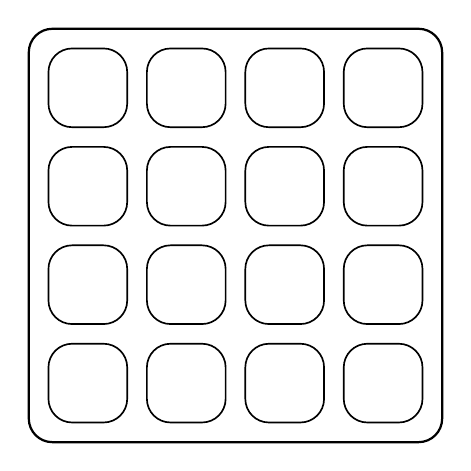
\begin{tikzpicture}
            \draw [rounded corners = 3mm, thick]
            (0,0) coordinate (tmp)
            ++(\keypadSide,-\keypadSide) coordinate (tmp)
            (0,0) rectangle ++(\keypadSide,-\keypadSide)
            (0,0) coordinate (origin)
            ;
            \foreach \y in {0.25,1.5,...,5} {
                \foreach \x in {0.25,1.5,...,5} {
                    \draw [semithick, rounded corners = 3mm]
                    (origin) ++(\x,-\y) rectangle +(1,-1)
                    ;
                }
            }
        \end{tikzpicture}
    }
    %% bottom pins
    (#1-origin) ++(0,-\keypadSide)
    ++(0.75,-0.25) coordinate (#1-pin-01)
    ++(1.25,0) coordinate (#1-pin-02)
    ++(1.25,0) coordinate (#1-pin-03)
    ++(1.25,0) coordinate (#1-pin-04)
    %% right pins
    (#1-origin) ++(\keypadSide,0)
    ++(0.25,-0.75) coordinate (#1-pin-08)
    ++(0,-1.25) coordinate (#1-pin-07)
    ++(0,-1.25) coordinate (#1-pin-06)
    ++(0,-1.25) coordinate (#1-pin-05)
    %% top pins
    (#1-origin)
    ++(0.75,0.25) coordinate (#1-pin-12)
    ++(1.25,0) coordinate (#1-pin-11)
    ++(1.25,0) coordinate (#1-pin-10)
    ++(1.25,0) coordinate (#1-pin-09)
    %% left pins
    (#1-origin)
    ++(-0.25,-0.75) coordinate (#1-pin-13)
    ++(0,-1.25) coordinate (#1-pin-14)
    ++(0,-1.25) coordinate (#1-pin-15)
    ++(0,-1.25) coordinate (#1-pin-16)
    %% column pins
    (#1-pin-01) coordinate (#1-pin-c1)
    (#1-pin-02) coordinate (#1-pin-c2)
    (#1-pin-03) coordinate (#1-pin-c3)
    (#1-pin-04) coordinate (#1-pin-c4)
    %% row pins
    (#1-pin-13) coordinate (#1-pin-r1)
    (#1-pin-14) coordinate (#1-pin-r2)
    (#1-pin-15) coordinate (#1-pin-r3)
    (#1-pin-16) coordinate (#1-pin-r4)
    %% geo coordinates
    \markgeocoordinate {#1}
    {(#1-pin-12)} {(#1-pin-01)}
    {(#1-pin-16)} {(#1-pin-08)}
}

\ctikzsubcircuitactivate{spicKeypad}

\newcommand\ovrKeypadPinHoles[1] {
    (#1-pin-01) node [ocirc] {}
    (#1-pin-02) node [ocirc] {}
    (#1-pin-03) node [ocirc] {}
    (#1-pin-04) node [ocirc] {}
    (#1-pin-05) node [ocirc] {}
    (#1-pin-06) node [ocirc] {}
    (#1-pin-07) node [ocirc] {}
    (#1-pin-08) node [ocirc] {}
    (#1-pin-09) node [ocirc] {}
    (#1-pin-10) node [ocirc] {}
    (#1-pin-11) node [ocirc] {}
    (#1-pin-12) node [ocirc] {}
    (#1-pin-13) node [ocirc] {}
    (#1-pin-14) node [ocirc] {}
    (#1-pin-15) node [ocirc] {}
    (#1-pin-16) node [ocirc] {}
}

\newcommand\ovrKeypadRowColPinHoles[1] {
    %% columns
    (#1-pin-c1) node [ocirc] {}
    (#1-pin-c2) node [ocirc] {}
    (#1-pin-c3) node [ocirc] {}
    (#1-pin-c4) node [ocirc] {}
    %% rows
    (#1-pin-r1) node [ocirc] {}
    (#1-pin-r2) node [ocirc] {}
    (#1-pin-r3) node [ocirc] {}
    (#1-pin-r4) node [ocirc] {}
}
